% !TEX program = XeLaTeX
% !TEX encoding = UTF-8
\documentclass[UTF8,nofonts]{article}
%{ctexart}


%\setCJKmainfont[BoldFont=FandolSong-Bold.otf,ItalicFont=FandolKai-Regular.otf]{FandolSong-Regular.otf}
%\setCJKsansfont[BoldFont=FandolHei-Bold.otf]{FandolHei-Regular.otf}
%\setCJKmonofont{FandolFang-Regular.otf}

\usepackage{url}
\usepackage{cancel}
\usepackage{xspace}
\usepackage{graphicx}
\usepackage{multicol}
\usepackage{multirow}
\usepackage{subfig}
\usepackage{amsmath}
\usepackage{amssymb}
%\usepackage[a4paper, width=180mm, top=18mm, bottom=22mm, includeheadfoot]{geometry}
\usepackage[a4paper, width=140mm, top=18mm, bottom=22mm, includeheadfoot]{geometry}
\usepackage{booktabs}
\usepackage{array}
\usepackage{verbatim}
\usepackage{caption}
%\usepackage{natbib}
\usepackage{booktabs}
\usepackage{float}
\usepackage{pdflscape}
\usepackage{mathtools}
\usepackage[usenames, dvipsnames]{xcolor}
\usepackage{afterpage}
\usepackage{pgf}
\usepackage{tikz}
\usepackage{dirtree}
\usepackage{amsfonts}
\usepackage{tkz-graph}


\newtheorem{definition}{Definition}[section]
\newtheorem{theorem}{Theorem}[section]
\newtheorem{lemma}{Lemma}
\newtheorem{proof}{Proof} [section]



\usepackage[toc, page, title, titletoc, header]{appendix}
\usepackage{marginnote}
\usepackage{tablefootnote}

%\renewcommand\appendixname{附\ 录}
%\renewcommand\appendixpagename{附\ 录}
%\renewcommand\appendixtocname{附\ 录}
\renewcommand\abstractname{Abstract}


\usepackage{perpage} %the perpage package
\MakePerPage{footnote} %the perpage package command

\usetikzlibrary{shapes.geometric}%
\usepackage{color}
%\usepackage[pages=some, placement=top]{background}
\usepackage{eso-pic}

\title{\textbf{LOOPRING}\\\textbf{Decentralized Token Exchange Protocol}\\v1.22}
\author{
  daniel@loopring.org\\
  jay@loopring.org\\
  alex@loopring.org\\ 
  \\
  \textit{Loopring Project Ltd}\\
%  \textit{http://Loopring.io}\\
  \textit{foundation@loopring.org}\\
 }

\makeatletter
\def\CTEX@section@format{\Large\bfseries}
\makeatother

\makeatletter
\newenvironment{tablehere}
 {\def\@captype{table}}
 {}

\newenvironment{figurehere}
 {\def\@captype{figure}}
 {}
\makeatother
%
%\newcommand\BackgroundPic{%
%\put(0, 0){%
%\parbox[b][\paperheight]{\paperwidth}{%
%\vfill
%\centering
%
\includegraphics[width=\paperwidth, height=\paperheight, %
%%keepaspectratio]{images/background.jpg}%
%]{images/background.jpg}%
%\vfill
%}}}


\begin{document}
%\AddToShipoutPicture{\BackgroundPic}
\maketitle
This document is for informational purposes only and does not constitute an offer or solicitation to sell shares or securities. Any such offer or solicitation will be made only by means of a confidential offering memorandum and in accordance with the terms of all applicable securities and other laws.



\begin{abstract}
Loopring is an open, multilateral token exchange protocol, for decentralized exchange on the Ethereum blockchain. Loopring is intended to serve as common building block with open standards, driving interoperability among decentralized applications (DAPPs) that incorporate exchange functionality. Trades are executed by a system of Ethereum smart contracts that are publicly accessible, free to use, and that any dApp can hook into.
\end{abstract}

\newpage

\tableofcontents
\newpage

\section{Background\label{sec: background}}

Blockchain\cite{staff2016blockchains}\cite{swan2015blockchain} technology was created to facilitate the cryptocurrency Bitcoin\cite{nakamoto2008Bitcoin}. It was originally intended for use as a decentralized system to enforce financial agreements\cite{lamport1982byzantine}\cite{christidis2016blockchains}. The technology that underlies such agreements is able to spread into other transactions: trading stock, IP, purchase and sale of real estate, purchasing music, and much more. Both consortium blockchain and private blockchain have been developed and implemented during the last few years, however the value only exists within a closed set of entities. Conversely, fully public blockchain operates by having a large number of participants, resulting in trust through numbers. According to coinmarketcap.com stats, the total cryptocurrency market cap value has reached to 113 billions USD,  including 32 billions USD from Ethereum\cite{wood2014ethereum} on June 12, 2017.

Blockchain has a massive influence across many domains,  particulary in the finance sector. It is strongly believed that tokenization\cite{liu2016medical}\cite{christidis2016blockchains}\cite{swan2015blockchain} offers many solutions across these domains. Asset tokenization can reduce cost, and globalize the asset and increase the liquidation thereof. As this technology expands, an increase in dApps will arise that require the use of these different tokens. As a result, an open standard for exchanging tokens is critical to support this open economy.

A regular exchange platform is based on peer-to-peer IOUs, and blockchain technology. Firstly,  users need to deposit their money or tokens into an exchange's bank account or wallet. Then their account will be credited an IOU. Thus, users are in fact trading their IOU in the exchange. Users have to file a ticket when they want to withdraw or sell the tokens.

Multiple exchanges have faced problems in past years. In February 2014, the largest Bitcoin exchange "Mt. Gox" suspended trading,  closed its website and exchange service, and filed for bankruptcy protection from creditors\cite{mcmillan2014inside}. Mt. Gox announced that approximately 850,000 Bitcoins belonging to customers and the company were missing and likely stolen; an amount valued at more than \$450 million at the time. Research showed that less than 1 percent (7000 btc) of missing funds were lost due to attacks. In 2016, the Bitfinex Hack occured in which \$72 million in Bitcoin was stolen from customer's accounts. As such, it is evident how a lack of regulation and protection has been injurious toward Bitcoin and other cryptocurrencies across many regions. It also illustrates how centralized exchange platforms carry unavoidable risk.

Loopring epitomizes a protocol that facilitates a decentralized exchange mechanism of ERC20 tokens on the Ethereum blockchain to solve the aforementioned issues. One of the strengths of decentralization is that of mitigated risk, wherein tokens are not held by a central authority. Therefore, asset theft or confiscation is impossible, leading to greater trust between customers and exchanges at a very low cost. Additionally, this mechanism has no time or regional limitations, is highly transparent, and has traceable features. Such features lead to effecting transactions that are more liquidatable, and to minimize price spread.

\section{Market and Industry\label{sec: existingworks}}

Decentralized exchange protocols built on blockchain technology do already exist. Examples of these include Ripple, BitShares, Openledger, Bancor, and 0x.

Ripple\cite{schwartz2014ripple} is a real-time gross settlement system, currency exchange, and remittance network operated by Ripple (the company). Also called the Ripple Transaction Protocol (RTXP) or Ripple protocol, it is built upon a distributed open source Internet protocol known as the consensus ledger. Ripple's solution is built around an open, neutral protocol (Interledger Protocol or ILP\cite{thomas2015protocol}) to power payments across different ledgers and networks globally. It offers a cryptographically secure end-to-end payment flow with transaction immutability and information redundancy. Architected to fit within a bank's existing infrastructure, Ripple is designed to comply with risk, privacy, and compliance requirements.

BitShares\cite{schuhbitshares}\cite{schuh2015bitshares} is an industrial grade financial blockchain smart contract platform. The BitShares decentralized exchange - also known as "The DEX" is a next-generation cryptocurrency trading platform. The DEX is inherently decentralized, enabling one to trade the BitShares core token (BTS) and a range of trustless price-stable, market-pegged assets, such as bitUSD, bitCNY, bitBTC, bitGold, and others. These assets can all be traded with zero counter-party risk, putting the user in total control of funds. However, the Bitshares project has many limitations.

The OpenLedger Dex\cite{openledger} is a cryptocurrency exchange. It allows users to exchange Bitcoin into smartcoins and then withdraw the smartcoins and convert them into cash through PayPal, Ripple, or NanoCard. Additionally, Openledger relies greatly on the BitShares 2.0 platform and Graphene Toolkit's operation.

The Bancor\cite{bancor}\cite{hanson2012logarithmic} protocol enables built-in price discovery and a liquidity mechanism for tokens on smart contract blockchains. These "smart tokens" hold one or more other tokens in reserve and enable any party to instantly purchase or liquidate the smart token in exchange for any of its reserve tokens. This is done directly through the smart token's contract, at a continuously calculated price according to a formula which balances buy and sell volumes.

"0x"\cite{warren20170x} is a protocol that facilitates low friction peer-to-peer exchange of ERC20\cite{ERC20} tokens on the Ethereum blockchain. The protocol is intended to serve as an open standard and common building block driving interoperability among decentralized applications (dApps) that incorporate exchange functionality. Trades are executed by a system of Ethereum smart contracts that are publicly accessible, free to use and that any dApp can hook into. DApps built on top of the protocol can access public liquidity pools or create their own liquidity pool and charge transaction fees on the resulting volume. However, 0x protocol has limitations including  only being able to accept simple OTC orders, having an unclear competing mechanism among differenth exchanges, and lacking a protection mechanism for miners.

Taking in to account the advantages and limitations stated above, it is clear that centralized exchange still plays an important role in the cryptocurrency market at present. Nevertheless, Our team, inspired by both 0x protocol and payment channel, have conveived a new solution for a decentralized exchange protocol.


\section{Design Protocol\label{sec: protocol}}

\begin{center}
\begin{figurehere}
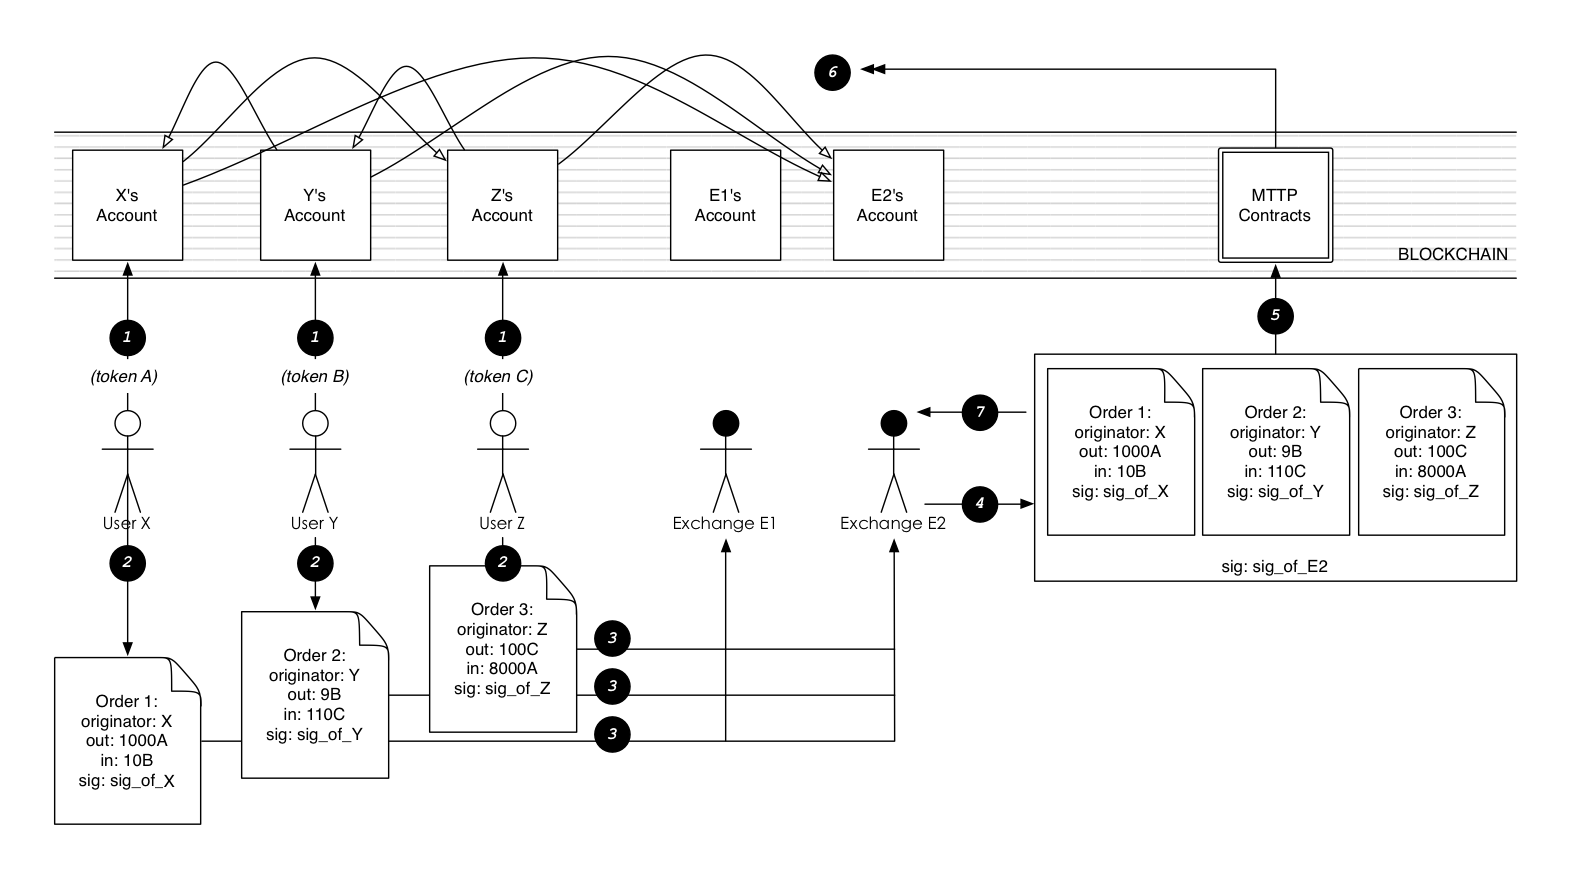
\includegraphics[height=8cm]{images/en_protocol.png}
\caption{Figure shows mix and match 3 orders}
\label{fig: Loopringrotocol}
\end{figurehere}
\end{center}

Figure 1 presents the general sequence of steps used for three parties transaction under Loopring:

\begin{enumerate}
 \item User X, Y, and Z authorize the Loopring smart contract to manipulate their accounts for token trading and exchanging. From the above figure, such a contract may transfer out 1000 token A from User X's account, transfer out 9 token B from User Y's account, and 100 token C from User Z's account;
 \item User X, Y, and Z place their own orders with signature using their private keys. Thus, all orders go into a medium and are ready to be exchanged - Order 1 is selling no more than 1000 token A and purchase no less than 10 token B; if the order is partially matched,  then the exchange rate between A to B should be no less than 1000/10=100.00 (selling tokens divided by purchasing tokens). Furthermore, to illustrate other parameters involved in chapter 3.7;
 \item User X, Y, and Z continue to send their order to one of the other multiple exchanges;
 \item After the exchange received three separated orders, they will replace them into a corresponding order-book, while updating a new block and calculating each orders status to match the set order - creating a loop we delineate as a ring exchange or matching exchange. Once all the orders are confirmed and successfully mix-matched;
 \item Exchange will send out a signature to the given Loopring smart contract address;
 \item Loopring smart contract will verify quadruple signatures in order to verify three orders closing. If closing is failed, then the contract will be terminated (certain exchange gas cost exempt); otherwise, Loopring smart contract needs to calculate the proceeds and cost for each users, then complete the token exchange --- as illustrated in the figure below. During each step, Loopring smart contract will use Loopring Registration Contract to calculate all the fees and discount before closing, the system will also need to use Loopring Stats Contract to update the database.

\begin{center}
\begin{figurehere}
\includegraphics[height=5cm]{images/en-Loopring-example.png}
\caption{Loopring:Match-Ring Settlement}
\label{fig:Loopringprotocol}
\end{figurehere}
\end{center}
  
  
 \item Exchange begins receiving new block and new data from the chain in order to upgrade the order-book then to mix-match new and existing orders.
\end{enumerate}


\subsection{Definition of Symbol}

Symbols are defined as follows.
\[
\begin{split}
&C_{i}\text{: \ }\text{stands for the $i$-th token.}\\
&O_{i\rightarrow j}\text{: \ }\text{stands for an order selling token $C_{i}$ for token $C_{j}$ .}\\
&s_{i\rightarrow j}\text{: \ }\text{selling token upper limit in order $O_{i\rightarrow j}$.}\\
&b_{i\rightarrow j}\text{: \ }\text{buying token lower limit in order $O_{i\rightarrow j}$.}\\
&r_{i\rightarrow j}\text{: \ }\text{max exchange rate in order $O_{i\rightarrow j}$, which is $s_{i\rightarrow j} / b_{i\rightarrow j}$.}
\end{split}
\]


We underlined the symbols to place emphasis on their original numbers. For example $\overline{s}_{i\rightarrow j}$ and $\overline{b}_{i\rightarrow j}$ stands for the number of tokesn from the original order.

\subsection{Rate Immutability\label{sec: consistrate}}

Loopring demands that the max-return exchange rate in an order stay immutable until the order is closed: 
$s_{i\rightarrow j} / b_{i\rightarrow j} = \overline{s}_{i\rightarrow j}/ \overline{b}_{i\rightarrow j}$. This guarantees that after an order is partially filled, the remaining order still satisfies the user's original intention.

\subsection{Order Reducibility\label{sec: reducibility}}


We can use token $C_j$ to connect two orders ( $O_{i\rightarrow j}$ and $O_{j\rightarrow k}$ ), regard it as one single order for selling token $Ci$ for buying token $C_k$. we use $O_{i\rightarrow j\rightarrow k}$ to represent this order. This order $O_{i\rightarrow k}$'s properties can be calculated as: 

\begin{equation}
s_{i\rightarrow j\rightarrow k}=min(b_{i\rightarrow j}, s_{j\rightarrow k}) \cdot r_{i\rightarrow j}
\end{equation}

\begin{equation}
b_{i\rightarrow j\rightarrow k}=min(b_{i\rightarrow j}, s_{j\rightarrow k}) / r_{j\rightarrow k}
\end{equation}

\begin{equation}
r_{i\rightarrow j\rightarrow k}= r_{i\rightarrow j}\cdot r_{j\rightarrow k}
\end{equation}


Here we introduce a concept of order-chain. It contains two or more orders, each orders selling token is the following orders purchasing token except the last one in the chain. Additionally, final orders purchasing token should be different from the first orders selling token (otherwise it will become a ring).

\[ s_{0\rightarrow ...\rightarrow n} =
 \begin{cases}
  s_{0\rightarrow 1}   & \quad \text{as } n \text{ = 1}\\
  min(b_{0\rightarrow ...\rightarrow n-1}, s_{n-1\rightarrow n}) \cdot r_{0\rightarrow ...\rightarrow n-1} & \quad \text{as\ } n \text{ $>$ 1}\\
 \end{cases}
\]

\[ b_{0\rightarrow ...\rightarrow n} =
 \begin{cases}
  b_{0\rightarrow 1}   & \quad \text{as } n \text{ = 1}\\
  min(b_{0\rightarrow ...\rightarrow n-1}, s_{n-1\rightarrow n}) / r_{n-1\rightarrow n} & \quad \text{as\ } n \text{ $>$ 1}\\
 \end{cases}
\]


\[ r_{0\rightarrow ...\rightarrow n} = \prod_{i=0}^{n-1}{r_{i\rightarrow i+1}}
\]


\subsection{Match-Ring}

Most, if not all, centralized exchanges match orders from the two sides of a trading pair. Loopring, however, involves detecting a ring of orders that may involve multiple tokens/currencies. With one order Match-Ring, multiple orders can be filled instantly.

\begin{definition}[Match-Ring] Let $C_{0}$, $C_{1}$, $\cdots$, $C_{n-1}$ be $n$ different kinds of token, $O_{0\rightarrow 1}$, $\cdots$, $O_{i\rightarrow i\oplus 1}$, $\cdots$, $O_{n-1 \rightarrow 0}$ be $n$ orders. Those orders can form a ring for trading:
$$O_{0\rightarrow 1} \rightarrow \cdots \rightarrow O_{i\rightarrow i\oplus 1} \rightarrow \cdots \rightarrow O_{n-1\rightarrow 0} \text{, }$$
where $n$ is the length of the ring, and $i\oplus 1 \equiv i+1 \mod n$.
\end{definition}

Once the prices match the orders under circumstance, we could start to complete trading in this circle.

\subsubsection{Price\label{sec: matchprice}}
We will introduce an example for a better understanding of the price mechanism. Assume three kinds of token are $C_{0}$, $C_{1}$ and $C_{2}$, three separated orders: $O_{0\rightarrow 1}$, $O_{1 \rightarrow 2}$ and $O_{2 \rightarrow 0}$. Easy to approve: if and only if $r_{0 \rightarrow 1} \cdot r_{1 \rightarrow 2}\cdot r_{2 \rightarrow 0} = 1$,  all three orders could be filled using their respective exchange rate; If $r_{0 \rightarrow 1} \cdot r_{1 \rightarrow 2}\cdot r_{2 \rightarrow 0} > 1$, all these orders can be filled using a rate lower than their implicit max exchange rate. We named the first situation as \texttt{original-price matching}, the second as \texttt{discount-price matching}.

According to Loopring protocol, each order in the ring would share the same rate (price) discount. For instance, if the discounted rate is $\gamma$, then the price for each order will be:
$r_{0\rightarrow 1} \cdot (1-\gamma)$, $r_{1\rightarrow 2} \cdot (1-\gamma)$, $r_{2 \rightarrow 0} \cdot (1-\gamma)$, and satisfied: 
\begin{equation}
r_{0\rightarrow 1} \cdot (1-\gamma)\cdot r_{1\rightarrow 2} \cdot (1-\gamma) \cdot r_{2 \rightarrow 0} \cdot (1-\gamma) = 1
\end{equation}
We can find out: 
\begin{equation*}
\gamma = 1- \frac{1}{\sqrt[3]{r_{0\rightarrow 1} \cdot r_{1\rightarrow 2} \cdot r_{2\rightarrow 0}}}\text{.}
\end{equation*}
In the other circumstance, if transaction cross $n$ orders, the \texttt{discount} is: 
\begin{equation*}
\gamma = 1- \frac{1}{\sqrt[n]{\prod_{i=0}^{n-1} r^i}} \text{,}
\end{equation*}
where $r^i$ is the order turnover rate of $i$-th order. Obviously, only when the discount rate is $\gamma \ge 0$, these orders can be filled; and the $i$-th order's $O^i$ actual exchange rate $\hat{r^i} = r^i \cdot (1-\gamma)$, $\hat{r^i}\le r^i$.

%在章节\ref{sec: fee}中, 我们还会详细介绍交易所通过Loopring代币抵押的原因和细节, 最终的结果是每个交易都被迫给自己的撮合的实际兑换率打个折扣, 即\texttt{交易所折扣}.假交易所$X$的交易所折扣为$\mu$, 那么由该交易所撮合是, 最后的实际成交兑换率为: $\hat{r^i} = r^i \cdot (1-\gamma) \cdot (1-\mu)$


\subsubsection{Fill Volume\label{sec: matchquantity}}

finding the lowest value order can help to figure out the fill volume for each order. For instance, if the $i$-th order is the lowest value order, then the number of tokens sold from each order $\hat{s}$ and number of tokens purchased $\hat{b}$ from each order can be calculated as:

\[
\begin{split}
&\hat{s}^{i}=\overline{s}_i\text{, } \hat{b}^{i}=\hat{s}^{i}/ \hat{r}^i\text{, }\text{;}\\
&\hat{s}^{i\oplus 1}=\hat{b}^i\text{, } \hat{b}^{i\oplus 1}=\hat{s}^{i\oplus 1}/ \hat{r}^{i\oplus 1}\text{;}\\
&\hat{s}^{i\oplus 2}=\hat{b}^{i\oplus 2}\text{, } \hat{b}^{i\oplus 2}=\hat{s}^{i\oplus 2}/ \hat{r}^{i\oplus 2}\text{;}\\
& ...
%\text{.}
\end{split}
\]
where $\overline{s}_i$ is the the balance left after order partially filled.

During implementation we can safely assume any order in the ring to have the lowest value, then iterate through the ring at most twice to calculate each orders fill volume. 

\subsubsection{Cost and Fee\label{sec: fee}}

Exchanges normally charge a transaction fee. For instance, we assume the fee will be calculated in Loopring token $LRC$, order ID is $i$ and total fee for completing the transaction is $m^i$: 

\begin{equation*}
f^i = b^i \cdot m^i / \overline{b^i}
\end{equation*}


In order to encourage an exchange to offer best rate for users, Loopring would distribute profit from \texttt{cost saving} to the given exchange. as an order $O^i$,  if price for purchasing is $b^i$( $b^i \le \overline{b^i}$ ),  then we define the saving cost form as: 

\begin{equation*}
\Delta^i = b^i \cdot r^i \cdot \gamma
\end{equation*}

If Loopring requires every order to set up a saving cost distributing rate $\theta^i$, and minimum distributing ratio is $\Theta$. Then order $O^i$ should pay to exchange: 


\begin{equation*}
f^i = \Delta^i \cdot \Theta = b^i \cdot r^i \cdot \gamma \cdot \Theta
\end{equation*}

Income from cost saving among each matching trade is explicated by:

\begin{equation*}
F = \sum^{n-1}_{i=0} b^i \cdot r^i \cdot \gamma \cdot \Theta
\end{equation*}

In order to encourage $LRC$ usage, if the order has no preset token fee $m^i$, or $m^i=0$, then the actual ratio is 100\% regardless of the relevant hash in this order. If none of the order has set up this rate $\Theta=100\%$, then all proceeds from the saving will go to the exchange.

In the next chapter we will introduce a token pledge policy, and explain how the smart contract will list out each exchanges depositing tokens and rank them up. It will also calculate a \texttt{mandatory discount cost} for each exchange, $\lambda$. This figure will affect the total cost. Meanwhile, an exchange can also offer a discount, $\eta$. Total cost for completion of a full trade: 

\begin{equation*}
F =(1-\lambda)\cdot (1-\eta) \cdot \sum^{n-1}_{i=0} (b^i \cdot r^i \cdot \gamma \cdot \Theta + b^i \cdot m^i / \overline{b^i})
\end{equation*}


\subsubsection{Fee Discount}
Loopring requires an exchange platform to offer a discount for each transaction. The discount fee is dependent upon the number of deposited token $LRC$. The higher the rank, the lower the charged fee. For example rank $n$'s cost will be:

$$\lambda_{n} = 0.05\cdot(\ln (n+e-1) - 1)\text{.}$$
Details below:


\begin{table}[hbt]
 \centering
\begin{tabular}{p{3.5cm}|p{3cm}} %设置了每一列的宽度, 强制转换.
Deposit Ranking $n$ & cost for discount $\lambda$ \\ %用&来分隔单元格的内容 \\表示进入下一行
  \hline
1 & 0\%\\
\hline
2 & $1.57\%$\\
\hline
10 & $7.31\%$\\
\hline
20 & $10.39\%$\\
\hline
99 &$18.06\%$\\
\hline
100 &$18.11\%$\\
\hline
1000 &$29.55\%$\\
\hline
1001 &$30.00\%^*$\\
 \end{tabular}
\caption{Deposit $LRC$ Ranking and cost for discount} %显示表格的标题
\end{table}


For those exchanges ranked under 1001 and those undeposited exchanges, 30\% cost will apply.

Figure \ref{fig:discount} shows, $\lambda_{2} - \lambda_{1} \gg \lambda_{100} - \lambda_{99}$.

\begin{center}
\begin{figurehere}
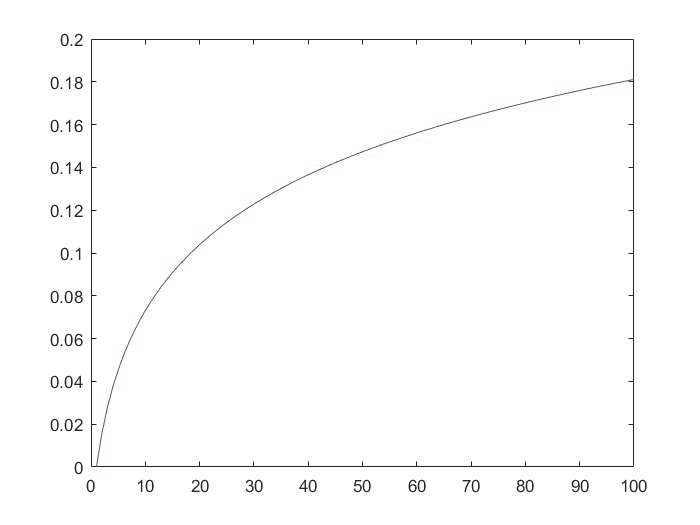
\includegraphics[height=8cm]{images/exchange-discount.png}

\caption{$LRC$ token deposit rank and cost for discount}
\label{fig:discount}

\end{figurehere}
\end{center}


\subsection{Fraud and Attack Protection}

\subsubsection{Exchange Covered Interest Arbitrage}

Loopring endevours to create a fair ecosystem and find a balance between customers (users) and exchanges. Firstly, we will explain how an exchange could archive a zero risk covered interest arbitrage.

Assume there are two orders $O_{a\rightarrow b}$, $O_{b\rightarrow a}$ that form a loop, $r_{a\rightarrow b} \cdot r_{b\rightarrow a} > 1$. An exchange can input three new orders between those two. $O_{b\rightarrow c}$, $O_{c\rightarrow d}$, $O_{d\rightarrow b}$, to create a five order loop,  $r_{a\rightarrow b} \cdot r_{b\rightarrow c} \cdot r_{c\rightarrow d}\cdot r_{d\rightarrow b}\cdot r_{b\rightarrow a} = 1$. An exchange could bring the possible cost down to zero once the transaction completed, implementing zero risk covered interest arbitrage
and $O_{b\rightarrow c}\rightarrow O_{c\rightarrow d}\rightarrow O_{d\rightarrow b}$. In order to stop these parameters, Loopring requires: {\bfseries a verified loop cannot create a further sub-loop to continue trading}.

\subsubsection{Denial-of-Service}

Loopring allows exchanges to selectively handle orders. An exchange can set up their own criteria and may choose to hide or reveal these criteria. Therefor Loopring does not see denial of service as a form of unethical behavior.

\subsubsection{Massive Tiny Order Attack}
A user can send out a large amount of tiny orders to attack exchanges. Exchanges however, will reject most of these tiny orders because they do not yield satisfying profit when matched. As denial-of-service is not deemed as a form of attack, massive tiny order attack is not feasible.

\subsubsection{Insufficient Balance}

Malicious users may sign and spread out orders whose value inside the order is not zero but whose address actually has zero balance. This again is a not a good way to attack exchanges. Exchanges will monitor and notice that some orders actual balance is zero and update these orders states accordingly, then discard them.  

Exchanges do have to spend time to update order status, but can also choose to minimize these effort by, for example, blacklisting some addresses and drop all related orders.

\subsubsection{Ring Filch}

A devient exchange could monitor all unconfirmed Match-Rings and broadcast the same rings with their own digital signature. We call this Ring Filch. In order to prevent Ring Filch Loopring allows exchanges to use two steps in order to submit the order: 
\begin{itemize}
  \item Submit the hash of a Match-Ring, wait for confirmation.
  \item Submit the ring itself.
\end{itemize}
Hash rate:
$$h = H(r,  nonce)\text{, }$$
where $H()$ is a one-way hash function, $r$ is Match-Ring record. Hash Hash function contains a random number $nonce$.

\subsection{Market Depth\label{sec: marketdepth}}

Exchange do not need to offer market depth data. Under this ecosystem, it is possible for both single entities and corporations to possibly pool all unclosed orders into one instance of market depth data. We can ascertain trading data between any two ERC20 tokens according to the agreement in chapter 3.3.

\subsection{Data Structure\label{sec: dataformat}}

All the orders can be represented by using one data structure due to adopting OTC module. This data structure contains both a digital signature and all parameters. Before the signature, the parameter data is connected from the orders into a set of data, the order's hash is calculated by using Keccak SHA3 method, and then signed by using this account's private keys with ECDSA.


\begin{verbatim}
message Order {
 address protocol;
 address owner;
 address outToken;
 address inToken;
 uint256 outAmount;
 uint256 inAmount;
 unit256 expiration
 unit256 fee;
 uint8 savingShare;
 unit8 v;
 bytes32 r;
 bytes32 s;
}
\end{verbatim}

Though there is no indicated price from the order, we are still able to find out through the formula: $outAmount / inAmount$ to determine the exchange rate $r$. The actual exchange rate must be less than $r$. A user-friendly exchange should allow user to input $outAmount$, $inAmount$, selling and asking price, and use any two of those numbers in order to calculate the missing $outAmount$ or $outAmount$ figure.

Actual orders can be defined in two different ways: Definition A - transaction can be completed once the number of tokens sold reaches $outAmount$ ; Definition B - transaction can be completed once the number of tokens purchased reaches $inAmount$; Therefore, we can setup a quote for exchange and mix-matching contract to help to define the trade. At our initial version, we would support Definition A only.

Exchange could create a Match-Ring by using this data structure:
\begin{verbatim}
message MatchRing {
  Order[] orders;
  address feeRecipient;
  unit256 additionalDiscount;
  unit256 nonce;
  unit8 v;
  bytes32 r;
  bytes32 s;
}
\end{verbatim}


\subsection{Order Status\label{sec: orderstate}}


An rrder cannot be modified once it has been signed and announced. Data will be updated on the blockchain once the smart contract finds the matched order. Thus $inAmount$ and $outAmount$ will modified correspondingly with the updated price. If $inAmount / outAmount$ shows 0,  it means that the order has been fully closed. For example, if the user wants to cancel the order, a special request will be filed,  $inAmount / outAmount$ will be 0 to close the order. An expired order will not be updated on the blockchain - it can be tracked through the final cutting time. Therefore, we expect most of the orders will expire or be invalidated.

\subsection{Smart Contracts\label{sec: contracts}}

Loopring consists of many smart contracts, including:

\begin{itemize}
 \item \textbf{Mix-Matched Contract} is responsible for ensuring each order status in the loop, calculating the price and volume,  transferring and interaction with other smart contracts, API for Loopring;
 \item  \textbf{Order Contract} updates order database and support cancelling policy;
 \item \textbf{Registration Contract} maintains and upgrades service for exchanges who accepted Loopring, support the token deposit from exchange and defaulted parameters backup;
 \item \textbf{Stats Contact} calculates the exchange volume and price between two tokens.

\end{itemize}

\begin{comment}
\subsection{支持ENS\label{sec: registration}}

\end{comment}

\section{Protocol Token \label{sec: protocoltoken}}


We will issue a token based on ERC20 Ethereum Token Standard called $LRC$ (displays in italics).


\subsection{Token Application}

$LRC$ will be use in the following areas:

\begin{itemize}
 \item \textbf{Gas Fees} --- $LRC$ can be paid as transaction fee for exchange. It will be simple and productive for the exchange to calculate all the cost in $LRC$. Same as request sender and receiver. We have mention this from previous chapter\ref{sec: fee}.
 \item \textbf{Deposit for Exchange Registration} --- The decentralized exchange mechanism has no limits on location or time. Consequently, exchanges with a high turnover would receive more orders and get more users. As a result of this, we have designed a policy for such exchanges that allow them to use $LRC$ to deposit into a smart contract in order to increase the exchanges credibility. Moreover, it can also protect users from certain adverse circumstances.
\end{itemize}

\subsection{Decentralized Governance}
Regulation has been updated as well as the exchanges mechanism. Any $LRC$ holders have the voting power $S$, and number of the pledging $N$ and pledging time $CoinAge$
$$S = f(N,  CoinAge)\text{, }$$
where $CoinAge = H_{c}-H_{s}$. Joining CoinAge aids to protect customers from speculation.

The decentralized mechanism includes token registration, exchange registration, stat hash, deposit scale, maximum length, discount hash, subcontract address.
 \begin{itemize}
   \item \textbf{token registration} Loopring would adjust token; low trading volume will be eliminated and new popular token will be replaced. All the adjustments have to be recorded on smart contract.
  \item \textbf{exchange registration} Only those exchanges that accept Loopring would allow trading to begin.
   \item \textbf{stat hash} Data will increase to a certain amount after a long period of operation. The more data exchanges have, the more accurate the system computation ability will be.
  \item \textbf{deposit scale} Deposit for each exchange should be measurable. if the amount is huge, the liquidation gets worse; verse vice.
   \item \textbf{maximum length} Technically, more orders can create more profit, however the risk of failure also increases, as well as the trading cost.
   \item \textbf{discount hash} Discount hash will be adjust with the market. The below figure shows  normal market (represented by the blue line), supply market (represented by the blue line), and the demand market (represented by the red line ).
\begin{center}
\begin{figurehere}
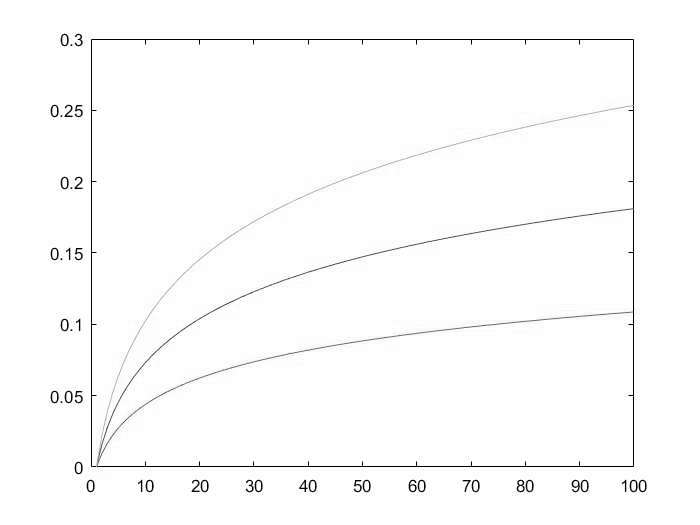
\includegraphics[height=10cm]{images/rate_adjust.jpg}
\caption{discount rate after adjustment}
\label{fig: dischargeRateAdjust}
\end{figurehere}
\end{center}

   \item \textbf{subcontract address} If Loopring exchange is based on the Ethereum ecosystem, then the smart contract cannot be modified. Therefore, one must update Loopring's subcontract in order to modify the subcontract address.
 \end{itemize}

%\footnotemark

\subsection{Token's Liquidability}

Loopring's token is based on ERC20 Ethereum Token Standard and can be liquidated through a Loopring smart contract. This means that LRC trading can be done through a centralized exchange. All the ERC20 Ethereum tokens can be exchanged to LRC token (assume pre-order is LRC, with zero fee) by adopting Loopring's decentralized mechanism.


\section{Exchange\label{sec: exchange}}

An exchange is unable to guarantee all transactions could make profit after adopting Loopring. The first reason is a high operating cost. Secondly, high expectation cannot match the actual outcome. There are few other reasons that would cause this saturation. Overall,  both the exchange platform and other parties have a reciprocal relationship: the exchange looks for a profitable order, while order senders look for an exchange with the lowest fee.
An exchange is not responsible for users ERC20 token after accepting Loopring. The workload has moved from money deposit, withdrawal,  and internal virtual account management, to mix-matched order service. Meanwhile, for the users, Loopring does not require the customer to deposit or lock any asset, that means an asset has zero risk to get stolen. Concurrently, a single order can mix and match multiple trades. For Non ERC20 asset, an exchange can offer a asset tokenization service.

\subsection{Regular and Loopring Exchange Comparison}
In a regular exchange, the "Maker" sends an order, and the "Taker" receive this order. The exchange's price highly depends on the sender's end. Under Loopring circumstances, it has adopted an Over-The-Counter (OTC) module.
In the current market, there is a considerably high risk for users to trade in these platforms; there are no laws to regulate the exchange if they vanish. But with Loopring, users do not to deposit money to the exchange anymore. All the transactions will be made among a user's coin address.
Another feature for Loopring is that it changes the "Trading Pair" concept. Transactions can be completed with multiple parties, rather than two parties in current exchange scenarios.


\begin{table}[hbt]
  \centering
\begin{tabular}{p{5cm}|p{2.5cm}|p{2.5cm}} %设置了每一列的宽度,强制转换。
&Centralized Exchange & Loopring Exchange \\ %用&来分隔单元格的内容 \\表示进入下一行
    \hline
Deposit for the order& Yes & No \tablefootnote{Exchanges execute under Loopring ecosystem do not require any deposit - Tokens are kept in user's wallet, no transaction will be made before the full contract close. As a result, no account can be stolen, or asset lost risk.}\\
\hline
Frozen Account& Yes & No \tablefootnote{Loopring exchanges do not require freeze trading fund --- If a user partially or fully modifies the fund, the contract will be withdraw automatically.}\\
\hline
Deposit/Withdraw& Yes & No \tablefootnote{The sender's order can be distributed to multiple receivers to be partially or fully fulfilled under Loopring ecosystem.}\\
\hline

Internal Trading Risk& Yes & No\tablefootnote{All matching trades are based on smart contract on blockchain, data are immutable and transparent.}\\
\hline
Customer loss from exchange closing& Yes & No\tablefootnote{ Loopring exchanges are not responsible for tokenization, thus Loopring users will not be affected if an exchange becomes insolvent. For example, a blockchain account will not affected if mining is terminated. In conclusion, exchanges are responsible for matching trades. Loopring's smart contract will complete clearing and settlement, furthermore, assets are always kept in user’s blockchain account.}\\
\hline
Transaction is the main income& Yes & No\tablefootnote{Transaction fee is not a mainstream income for Loopring exchanges, mainstream comes from “profit of transaction cost saving”, because it can effectively encourage trade matching.}\\
\hline
Accept Fiat Money& Yes & Yes\tablefootnote{Loopring exchanges fully support asset tokenization, hence, it requires legitimate currency being tokenized on ERC20 standard.}\\
\hline
Can be traded among multiple exchanges& No & Yes \tablefootnote{Loopring allows multiple Loopring exchanges to partially or fully trade off one order at same time.}\\
\hline
Fairness for Maker and Taker& No & Yes \tablefootnote{Transaction price is closed to the balance price instead of being tendered to the maker’s offer price under Loopring protocol.}\\
\hline
Mix and Match Trading& No & Yes\tablefootnote{ Loopring exchanges’ multiple supporting feature can help sender to find the most profitable order.}\\
\hline
Supervision & Strong & Weak\tablefootnote{Loopring exchanges do not require a deposit. Clearing and settlement are made through the open source smart contract. Therefore, regulation is not necessary if there is no asset tokenization occurrence.}\\

  \end{tabular}

\caption{Contrast between centralized exchange and Loopring exchange} %显示表格的标题
\end{table}

%\footnotemark


\section{Summary\label{sec: summary}}

Loopring is a protocol that facilitates decentralized exchange of ERC20 tokens on the Ethereum blockchain. Loopring allows multi-token transaction exchange, as well as acceptance of exchange of liquidation on the blockchain under different circumstances. Loopring offers benefit to both users and exchanges by deferring risk from both parties in decentralized smart contracts, minimising fees and cost to create more profitable orders through ring-matching and order-sharing, and as a cross-platform protocol. Loopring protocol fits any ERC20 and smart contract blockchain platform. After many discussion,  our team will develop Loopring on the Ethereum blockchain.

\section{Acknowledgements\label{sec: acknowledgement}}

We would like to express our gratitude to our mentors, advisers and to the many people in the community that have been so welcoming and generous with their knowledge. In particular, we would like to thank Shuo Bai (from ChinaLedger); Professor Haibin Kan; Alex Cheng, Hongfei Da; Yin Cao; Jia Sheng; Xiaochuan Wu; Zhen Wang, Wei Yu, Nian Duan, Jun Xiao, Jiang Qian, Jiangxu Xiang, Yipeng Guo, Dahai Li, Kelvin Long, Huaxia Xia, Jun Ma, and Encephalo Path for reviewing and providing feedback on this work. We are also welcoming more feedback from community.

\newpage  
\bibliography{whitepaper}
\bibliographystyle{unsrt}

%\newpage
%
%\begin{appendices}
%\section{$LRC$ Token Crowdsale\label{sec: ico}}
%
%We plan to issue 100 million LRC token, 80 million tokens will be allocated to crowdsale participators, and the remaining 20 million tokens will be allocated to the foundation initiator for maintenance and development of the Loopring community over the next 5 years.
%
%ICO will start pre-sale to investors and crowdsale in 2017 July. We plan to raise XXXX ETH
%Initial spending plan;
%
%\begin{table}[hbt]
% \centering
% \begin{tabular}{l|c}
%   Purpose    & Percentage\\
%  \hline
% Tech Development  & 50\% \\
% Community Building & 20\% \\
% Marketing     & 15\% \\
% Legal and Law   & 15\% \\
% \end{tabular}
% \caption{ Plan for token expense}
%\end{table}
%
%
%
%Project ICO and Timetable
%\begin{table}[hbt]
% \centering
% \begin{tabular}{l|l}
%Time  & Target\\
%  \hline
% 2017/06 & Whitepaper release, Project start-off \\
% 2017/07 & Module Development Completion \\
% 2017/08 & Loopring open source committee(Foundation)set and Pre ICO closed \\
% 2017/08 & ICO schedule \\
% 2017/09 & ICO start \\
% 2017/10 & ICO close and release result \\
% 2017/11 & $LRC$Token IOU launch at exchange \\
% 2017/12 & Test $LRC$ token on ETH \\
% 2018/02 & Commencement \\
% 2018/04 & Issue $LRC$ token on ETC \\
% \end{tabular}
% \caption{Project Schedule}
%\end{table}
%
%\subsection{ETH/ETC Due-chain issue\label{sec: chains}}
%
%Alhough we only accept ETH as our ICO token, we also consider ETC token's potential on developing smart contract. Hence, we will issue our token $LRC$ on both Ethereum (ETH)and Ethereum Classic(ETC).
%
%
%\subsection{Risk Awareness\label{sec: risks}}
%
%Initial crypto-token offering (ICO) is a popular way for crowdsale, however it contains certain risks. Participators should be fully aware of all the potential risk and The Loopring Foundation hereby expressly disclaims its liability, and shall in no case be liable to any person, for: 
%\begin{itemize}
% \item any person's participation in the Campaign in violation of any anti-money laundering, counter-terrorism financing or other regulatory requirements that are imposed in any jurisdiction;
% \item any person's participation in the Campaign in violation of any representation, warranty, obligation, covenant or other provision under this prospectus, and the resulting failure or inability to retrieve his/her payment or to claim relevant purchased $LRC$ for Crowdsale;
% \item early termination of the Campaign for any reason;
% \item failure or abortion of the Quantum development and resulting failure to deliver the purchased $LRC$ for Crowdsale to the Purchasers;
% \item any risk factors disclosed in this Prospectus and any damage, loss, claim, liability, punishment, cost or other adverse impact that is caused by, associated with, in connection with, incidental to or consequential to that risk factor.
% \item if there is any separate agreement between a Purchaser and a Crowdsale Intermediary, this Prospectus shall take precedence over that agreement in all respects. The Loopring Foundation shall in no case be bound by, and hereby disclaims any liability under, the foregoing agreement.;
% \item failure or abortion of the Loopring development and resulting failure to deliver the purchased $LRC$ for crowdsale to the Purchasers;
%
%\end{itemize}
%
%
%
%\end{appendices}
\end{document}
